\documentclass[a4paper,14pt]{article} % тип документа
%\documentclass[14pt]{extreport}
\usepackage{extsizes} % Возможность сделать 14-й шрифт


\usepackage{geometry} % Простой способ задавать поля
\geometry{top=20mm}
\geometry{bottom=25mm}
\geometry{left=15mm}
\geometry{right=15mm}

\setcounter{section}{0}

%%%Библиотеки
%\usepackage[warn]{mathtext}
%\usepackage[T2A]{fontenc} % кодировка
\usepackage[utf8]{inputenc} % кодировка исходного текста
\usepackage[english,russian]{babel} % локализация и переносы
\usepackage{caption}
\usepackage{listings}
\usepackage{amsmath,amsfonts,amssymb,amsthm,mathtools}
\usepackage{wasysym}
\usepackage{graphicx}%Вставка картинок правильная
\usepackage{float}%"Плавающие" картинки
\usepackage{wrapfig}%Обтекание фигур (таблиц, картинок и прочего)
\usepackage{fancyhdr} %загрузим пакет
\usepackage{lscape}
\usepackage{xcolor}
\usepackage{dsfont}
%\usepackage{indentfirst}
\usepackage[normalem]{ulem}
\usepackage{hyperref}




%%% DRAGON STUFF
\usepackage{scalerel}
\usepackage{mathtools}

\DeclareMathOperator*{\myint}{\ThisStyle{\rotatebox{25}{$\SavedStyle\!\int\!\!\!$}}}

\DeclareMathOperator*{\myoint}{\ThisStyle{\rotatebox{25}{$\SavedStyle\!\oint\!\!\!$}}}

\usepackage{scalerel}
\usepackage{graphicx}
%%% END 

%%%Конец библиотек

\newcommand{\drawsome}[1]{            % Для быстрой вставки картинок
    \begin{figure}[h!]
            \centering
            \includegraphics[scale=0.7]{#1}
            \label{fig:first}
    \end{figure}
}
\newcommand{\drawsomemedium}[1]{
    \begin{figure}[h!]
            \centering
            \includegraphics[scale=0.45]{#1}
            \label{fig:first}
    \end{figure}
}
\newcommand{\drawsomesmall}[1]{
    \begin{figure}[h!]
            \centering
            \includegraphics[scale=0.3]{#1}
            \label{fig:first}
    \end{figure}
}

%%%Настройка ссылок
\hypersetup
{
colorlinks=true,
linkcolor=blue,
filecolor=magenta,
urlcolor=blue
}
%%%Конец настройки ссылок


%%%Настройка колонтитулы
	\pagestyle{fancy}
	\fancyhead{}
	\fancyhead[L]{Домашнее задание}
	\fancyhead[R]{Крейнин Матвей, группа Б05-005}
	\fancyfoot{}
    \fancyfoot[C]{\thepage}
    \fancyfoot[R]{ТРЯП}
%%%конец настройки колонтитулы



\begin{document}
%%%%Начало документа%%%%

\section{Задание 4}
\subsection{Задача 1}
    R $=$ $(a(a|b))^{*}b$, я построил этот автомат по алгоритму, этапы построения по алгоритму прилагаю в форме черновика.
    
    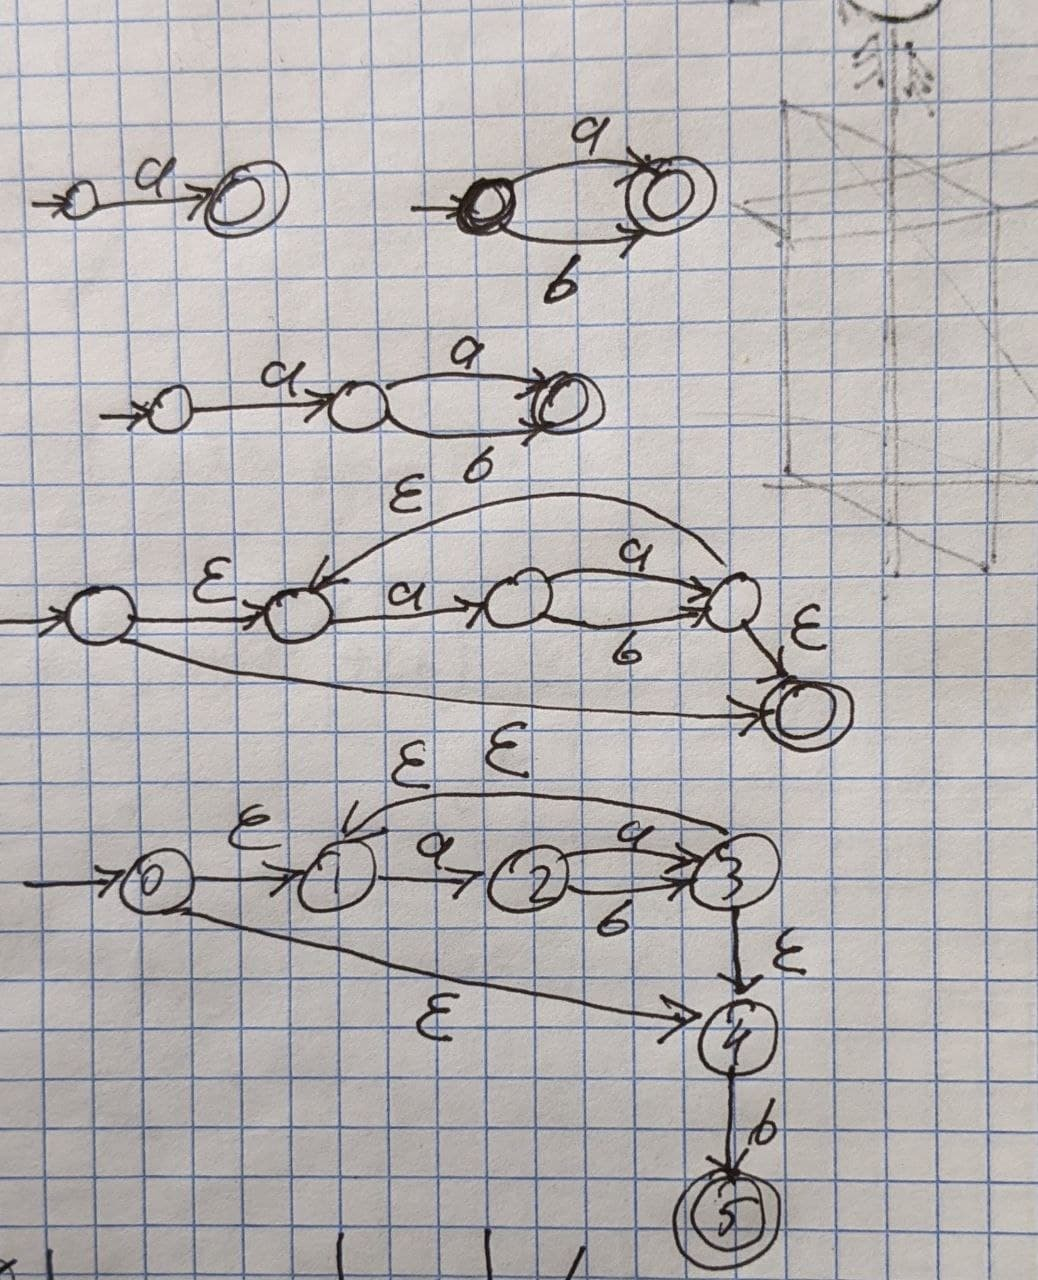
\includegraphics[scale=0.23]{02.jpg}
    
    А вот и сам автомат.

    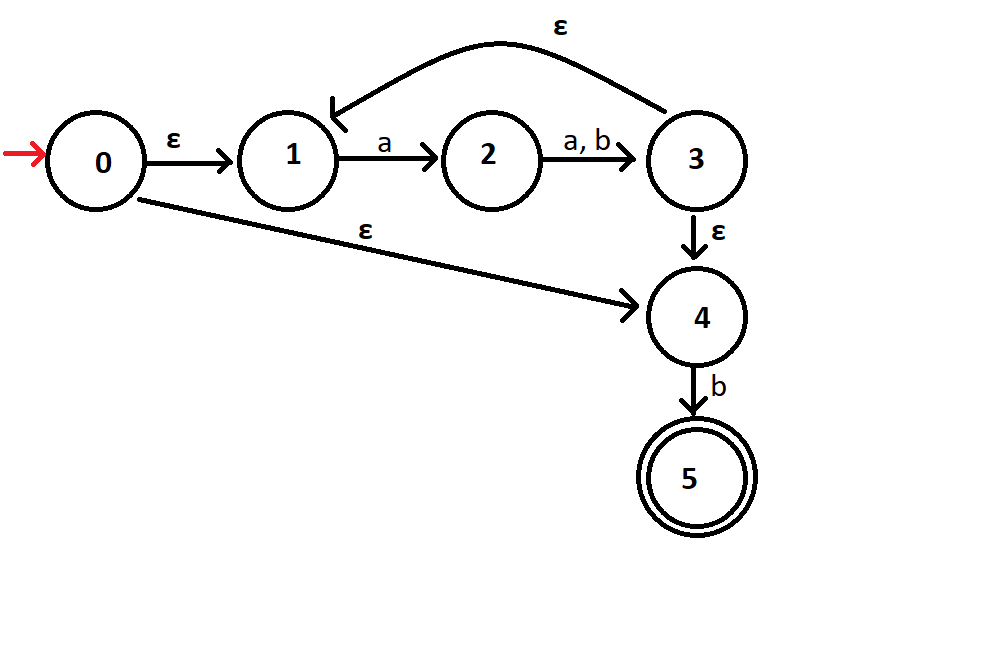
\includegraphics[scale=0.65]{01.png}
    
    
    \subsection{Задача 2}
    R $=$ $(a|b)^{*}abaab$, построил автомат по алгоритму в тетрадке, вот черновик.

    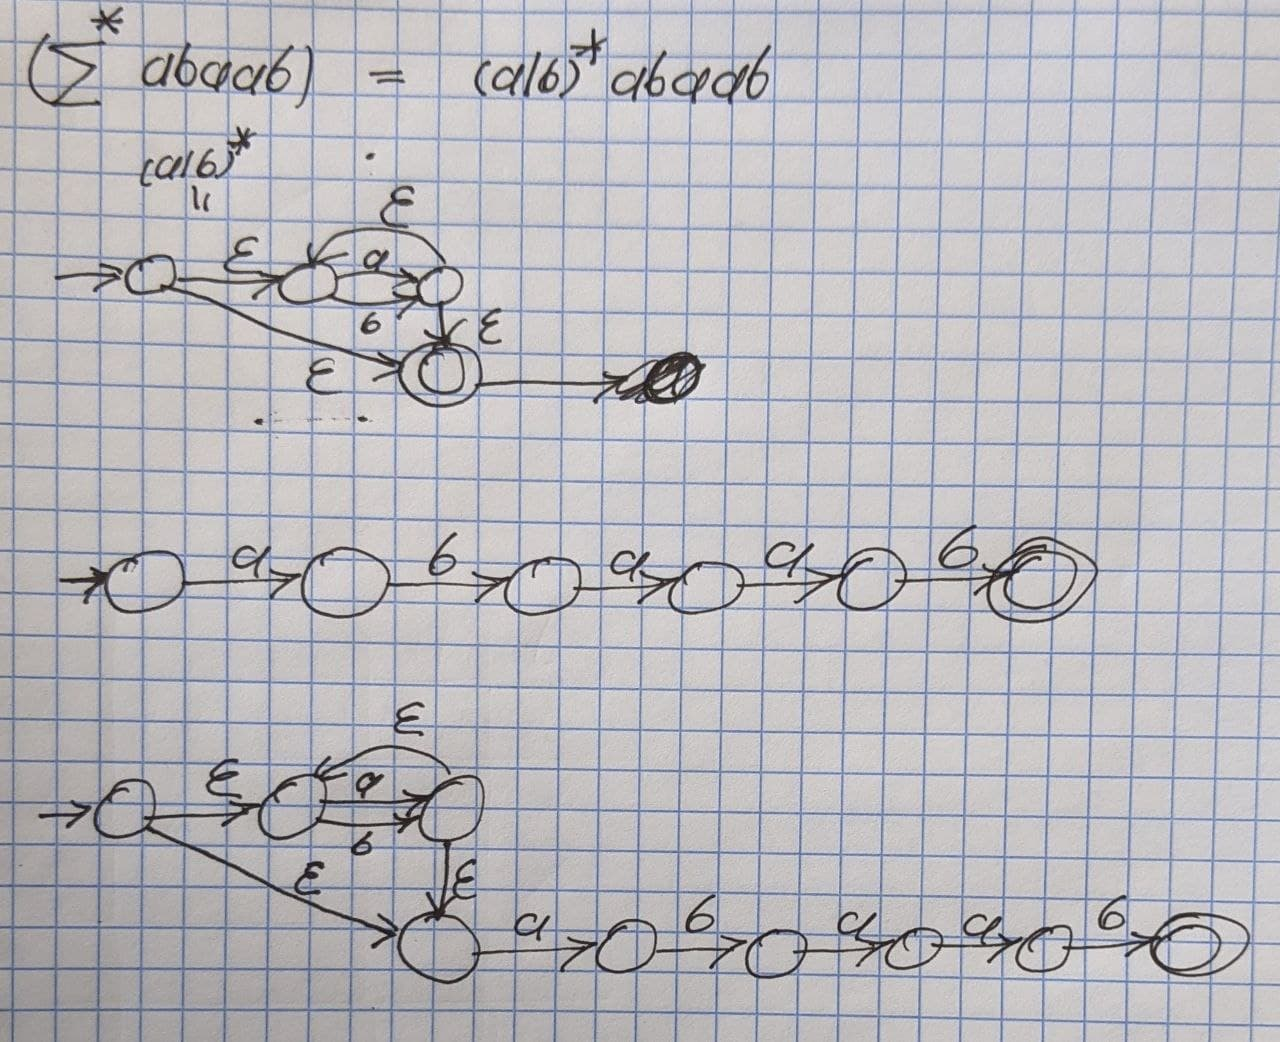
\includegraphics[scale=0.23]{04.jpg}
    
    А вот и сам автомат.

    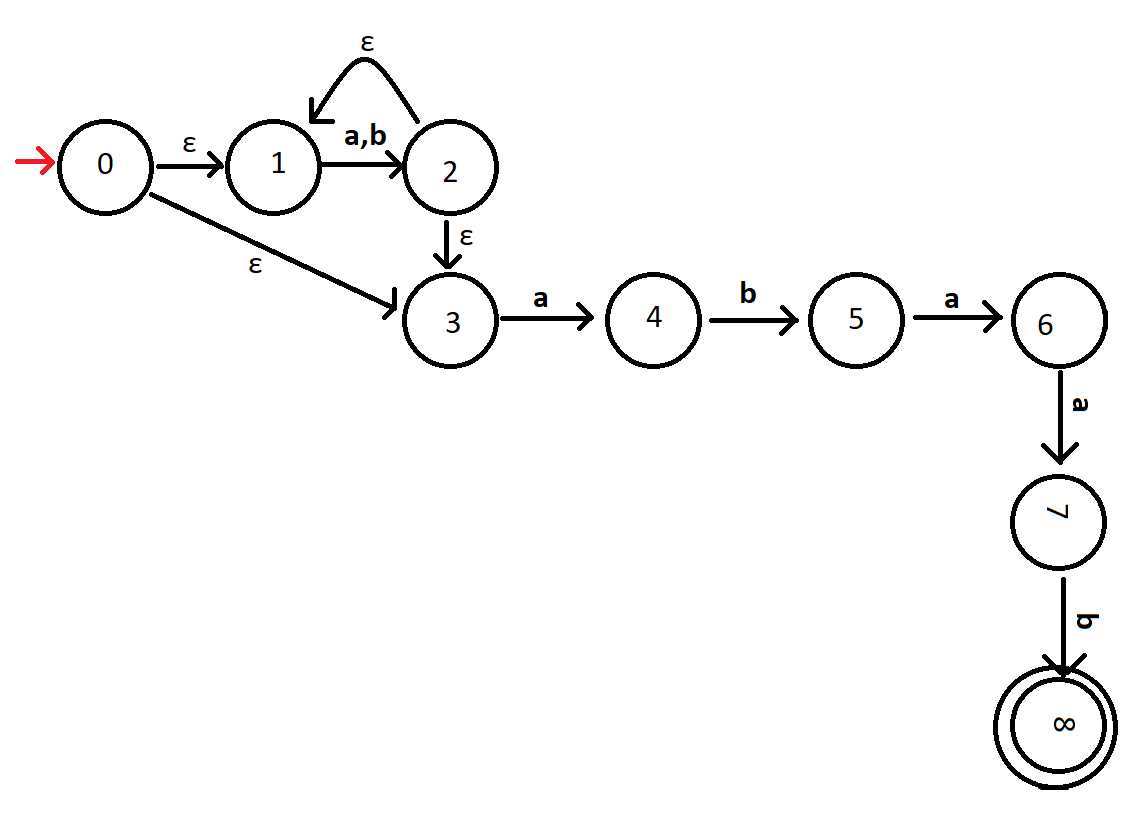
\includegraphics[scale=0.65]{03.png}

    \newpage
    \subsection{Задача 3}
    Составим таблицу, исходя из НКА из предыдущей задачи.

    \begin{tabular}{|l|l|l|l|}
    \hline
     & Куда можно перейти & \multicolumn{1}{c|}{a} & \multicolumn{1}{c|}{b} \\ \hline
    $\rightarrow$ $Q_0 $ & 1, 3               &  $Q_1$                      &  $Q_2$                      \\ \hline
    $Q_1 $ & 1, 2, 3, 4         &  $Q_1$                      &  $Q_3$                      \\ \hline
    $Q_2 $ & 1, 2, 3            &  $Q_1$                      &  $Q_2$                      \\ \hline
    $Q_3 $ & 1, 2, 3, 5         &  $Q_4$                      &  $Q_2$                      \\ \hline
    $Q_4 $ & 1, 2, 3, 4, 6      &  $Q_5$                      &  $Q_3$                      \\ \hline
    $Q_5 $ & 1, 2, 3, 7         &  $Q_2$                      &  $Q_6$                      \\ \hline
    $*Q_6 $ & 1, 2, 3, 8         &  $Q_1$                      &  $Q_2$                      \\ \hline
    \end{tabular}


    Теперь построим ДКА по этой таблице и получаем:

    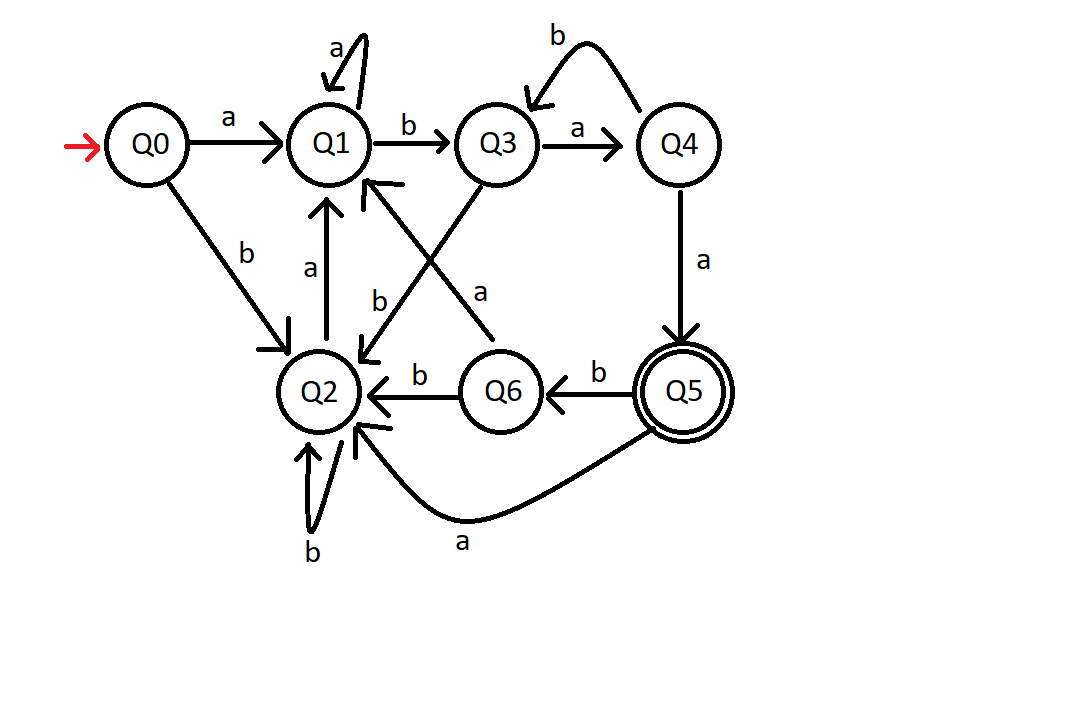
\includegraphics[scale=1]{05.png}

    \newpage
    \subsection{Задача 4}
    Да, для конечного языка L выполняется лемма о накачке.

    В любом конечном есть самое длинное слово, пусть это будет слово $\omega$, тогда возьмем за p = $|\omega| + 1$.
    Тогда получаем, что у нас нет такого слова из L, которое было бы длинее p (т.к. мы так выбрали p), сл-но получаем, что посылка в следовании ложна, сл-но следование получается истинным.

    \underline{Доказано}

    \subsection{Задача 5}
    \textbf{1.} $L = \{a^{2019n + 5} | n =0, 1, ...\} \cap \{a^{503k + 29} | k = 401, 402, ... \} \subseteq \{a^*\}$.
    Обозначим $L_1 = \{a^{2019n + 5} | n =0, 1, ...\}$ и $L_2 = \{a^{503k + 29} | k = 401, 402, ... \}$.
    
    Теперь рассмотрим $L_1$, он получается конкатенацией $\{a^{2019n} | n =0, 1, ...\}$ и $\{a^5\}$. Второе слагаемое получается конкатенацией 5 раз a, а это принадлежит регулярным языкам.
    А первое слагаемое получается как конкатенация $\{ a\}$ 2019 раз.
    $\{a^{2019n} \} \subseteq \{a\}^{*} $, тогда получается, что и первое слагаемое принадлежит регулярным языкам.
    А конкатенация двух регулярных языков тоже регулярный язык, получаем, что $L_1$ - регулярный язык.

    Теперь рассмотрим $L_2$, аналогично получаем, что $\{a\}^{29}$ - регулярный язык.
    $\{a^{201703n}\} \subseteq \{a\}^*$, аналогично получаем, что $L_2$ - регулярный язык.
    
    Т.к. REG замкнуто относительной пересечения получаем, что L тоже регулярный язык.

    \underline{Доказано}

    \textbf{2.} $L = \{a^{200n^2 + 1}| n = 1000, 1001, ...\}$
    Докажем, что для него не выполняется лемма о накачке.
    
    $\forall p \exists \omega \in L : |\omega| > p, \forall xyz = \omega ((y = \epsilon) \vee (|xy| > p) \vee (\exists i \geqslant 0 : xy^iz \notin L))$

    Рассмотрим два случая:

    1. Если p > $2 \cdot 10^8$, то тогда возьмем за $\omega = a^{200 \cdot 1000^2 + 1}$. 
    $\forall xyz = \omega, |y| \geqslant 1,$ $|xy^0z| = |\omega| - |y|$, $|xy^2z| = |\omega| + |y|$. 
    Пусть |y| = d, тогда если лемма была бы верна, то 
    $200n^2 +1 +d = 200(n+m)^2+1$ $\Rightarrow$ $d = 200(2n+m)m$
    и $200n^2+1-d = 200(n-k)^2 + 1$ $\Rightarrow$ $d = 200(2n+k)k$

    Откуда получаем, что m = k, но это невозможно т.к. $|(n-k)^2-n^2| \neq |(n+k)^2 -n^2|$, или же $2n+m+k = 0$, но n, m, k $\in \mathcal{N}$.
    Получается, что $xy^2z \notin L \vee xy^0z \notin L$, получается что при таких p не выполняется.

    2. Если p $\leqslant 2 \cdot 10^8$, то возьмем $\omega = a^{200*1000^2 + 1}$. $\forall xyz = \omega, |y| \geqslant 1, \exists i = 0 : |xy^iz| = |xz| < |\omega|$. Т.к. n = 1000, то $|xy^iz| \notin L$.
    Следовательно лемма не выполняется при таких p.

    А следовательно не выполняется ни при каких p, сл-но L - нерегулярен.
    
    \underline{Доказано}

    \subsection{Задача 6}
    \textbf{a)} Возьмем за R $= \invdiameter$, $R \in REG$, но $F \cup R = \invdiameter \ in REG$, из этого не следует, что $F \in REG$.
    Т.к. F может быть произвольным. 
    
    \underline{Ответ:} Нет, неверно.
    \newline
    \textbf{б)} $L_1$ = $F \cap R$, $L_2$ = $F \cap \overline{R}$.
    Заметим, что $L_1, L_2 \in REG$, и $L_1 \cup L_2 = (F \cap R) \cup (F \cap \overline{R}) = F \cap (R \cup \overline{R})$
    $= F \cap U = F$, но $L_1 \cup L_2 in REG$, сл-но $F \in REG$.
    
    \underline{Ответ:} Да, верно.
\end{document}